\documentclass[UTF8,fontset=ubuntu]{ctexart}
\usepackage{graphicx}
\usepackage{float}
\usepackage{amssymb}
\begin{document}
\begin{figure}[H]
	\centering
	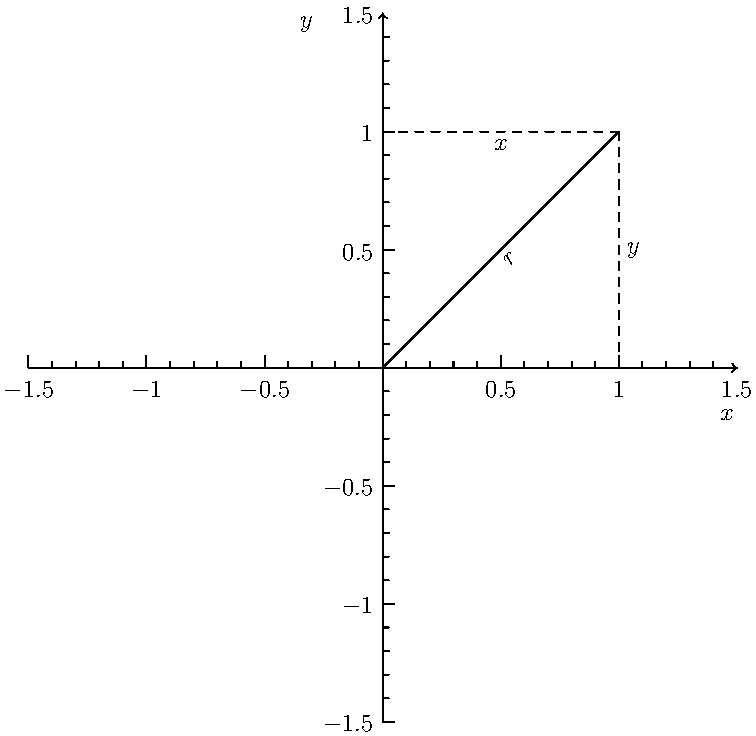
\includegraphics[scale=0.4]{quadrantal.pdf}
	\caption{象限图}
\end{figure}
常用三角函数公式\par
$sin(x)=\frac{y}{r}$\qquad$cos(x)=\frac{x}{r}$\qquad$tan(x)=\frac{y}{x}$\par
三角函数常见值分布\par
\begin{table}[H]
\centering
\begin{tabular}{c|c c c c c}
	\hline
	& 0 & $\frac{\pi}{6}$ & $\frac{\pi}{4}$ & $\frac{\pi}{3}$ & $\frac{\pi}{2}$\\
	\hline
	sin & 0 & $\frac{1}{2}$ & $\frac{1}{\sqrt{2}}$ & $\frac{\sqrt{3}}{2}$ & 1\\
	cos & 1 & $\frac{\sqrt{3}}{2}$ & $\frac{1}{\sqrt{2}}$ & $\frac{1}{2}$ & 0\\
	tan & 0 & $\frac{1}{\sqrt{3}}$ & 1 & $\sqrt{3}$ & $\bigstar$\\
	\hline
\end{tabular}
\end{table}
名词解释\par
弧度:旋转一周为$2\pi$\par
角度:旋转一周为$360^\circ$\par
参考角:射线与x轴形成的最小角度,该角度范围在$0\sim\pi/2$\par
三角函数值计算方式:将弧度限定在$0\sim2\pi$,并获得该弧度的参考角,然后根据角度所在象限,根据ASTC原理,获取函数值\par
毕达哥拉斯定理:
\[cos^2(x)+sin^2(x)=1\]
\end{document}
